%%%%%%%%%%%%%%%%%%%%%%%%%%%%%%%% 
\section{The DCS, DSS} 
\label{sec:detectors-fd-alt-dcs}

The slow control system for the far detector is part of a
continued progressive prototyping effort aiming at developing a
control system dedicated to multi-ton liquid argon double phase
detectors. It has been designed in the framework of the LAGUNA-LBNO design study and the WA105 experiment following the successful example and
the expertise developed in the context of the ArDM experiment  \cite{Badertscher:2013ygt}
which is currently operating 1 ton of liquid argon in an underground
laboratory (LSC, Spain) but it is introducing for the first time the use of National Instruments
compact RIO modules for acquisition of all the physical quantities of
interest. In Figure~\ref{fig:NI_proto} a rack prepared forthe WA105  $3 \times 1 \times 1$ $m^2$ prototype and ready to be tested at CERN.

 The slow control system of the far detector and $3 \times 1 \times 1$ $m^2$ prototype detectors is designed to monitor:
\begin{itemize}
  \item temperature through platinum resistors,
  \item pressure with commercial piezoelectric sensors,
  \item liquid argon level with custom made capacitive sensors and electronics,
  \item deformation of materials with resistive strain gauge
\end{itemize} 

inside the tank; moreover it provides the hardware
infrastructures needed to monitor traces of O2, N2 and H2O impurity in the tank, monitor and control of high
and low voltage power supplies, heaters, lighting system, vision
system and will interfaces with the cryogenic system and with the
motorized system to control the positioning of each single module of the Charge Readout Plane. 


\begin{cdrfigure}[Slow Control prototype rack]{NI_proto}{The rack is a prototype of the entire Control System; it  embeds modules for resistive temperature sensors, pressure  sensors, strain gauges, liquid argon level meters, control for  heaters. On the upper part a redundant 24 V power supply provides
 fault tolerant power to the National Instrument controller and modules. Calibration of modules and sensors is ongoing.}
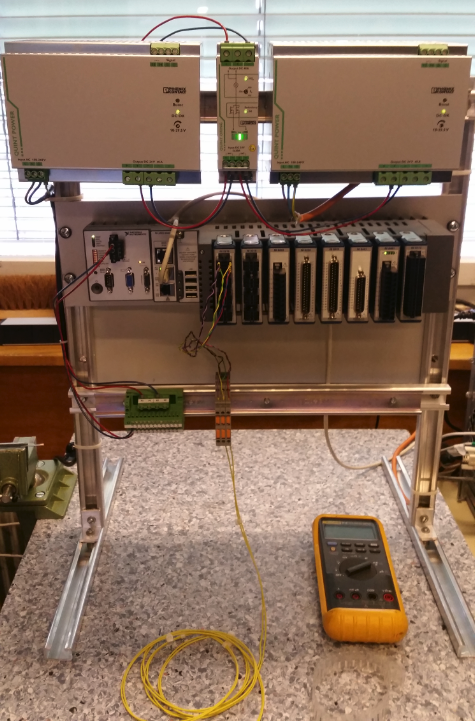
\includegraphics[scale=0.2, angle=0]{rack_2.jpg}
\end{cdrfigure}

 The entire control system will be monitored through a single LabView  interface which will implement together with the required sensor
 calibration, control of the actuators and the platform for vision  system inside and outside the tank. The overlying supervisory level
 will be implemented in UNICOS and will provide an interface to the  operator for monitoring of all the quantities and handling of alarms,
 as commonly done in all CERN experiments.  

As already detailed in the section about Charge Readout Plane, the charge readout system of the far detector is modularised in units of 4$\times$4 m$^2$ CRPs; each 4$\times$4 m$^2$ CRP is an independent detector, hence its instrumentation can be thought independently too. A complete list of the sensors which are been foreseen for both the 4$\times$4 m$^2$ far detector module and $3 \times 1 \times 1$ $m^2$ prototype detectors is provided in Table~\ref{fig:sc_sensors}.  The numbers presented for the far detector are hence an estimate taking in account the sensors we are installing in the $3 \times 1 \times 1$ $m^2$ prototype and they are not yet final.
\\ Regarding the sensors and instrumentation foreseen for the $3 \times 1 \times 1$ $m^2$ prototype this list has determined the design of the custom made feedthrough, so called Slow Control Feedthrough based on the use of weldable connectors for High Vacuum and shown in Figure~\ref{fig:SC_flange}.

\begin{cdrfigure}[Slow control feedthroughs]{SC_flange}{The 3 SCFT providing weldable connectors for all the instrumentation inside the tank. The number of sensors per module in the far detector will be drastically reduced.}
   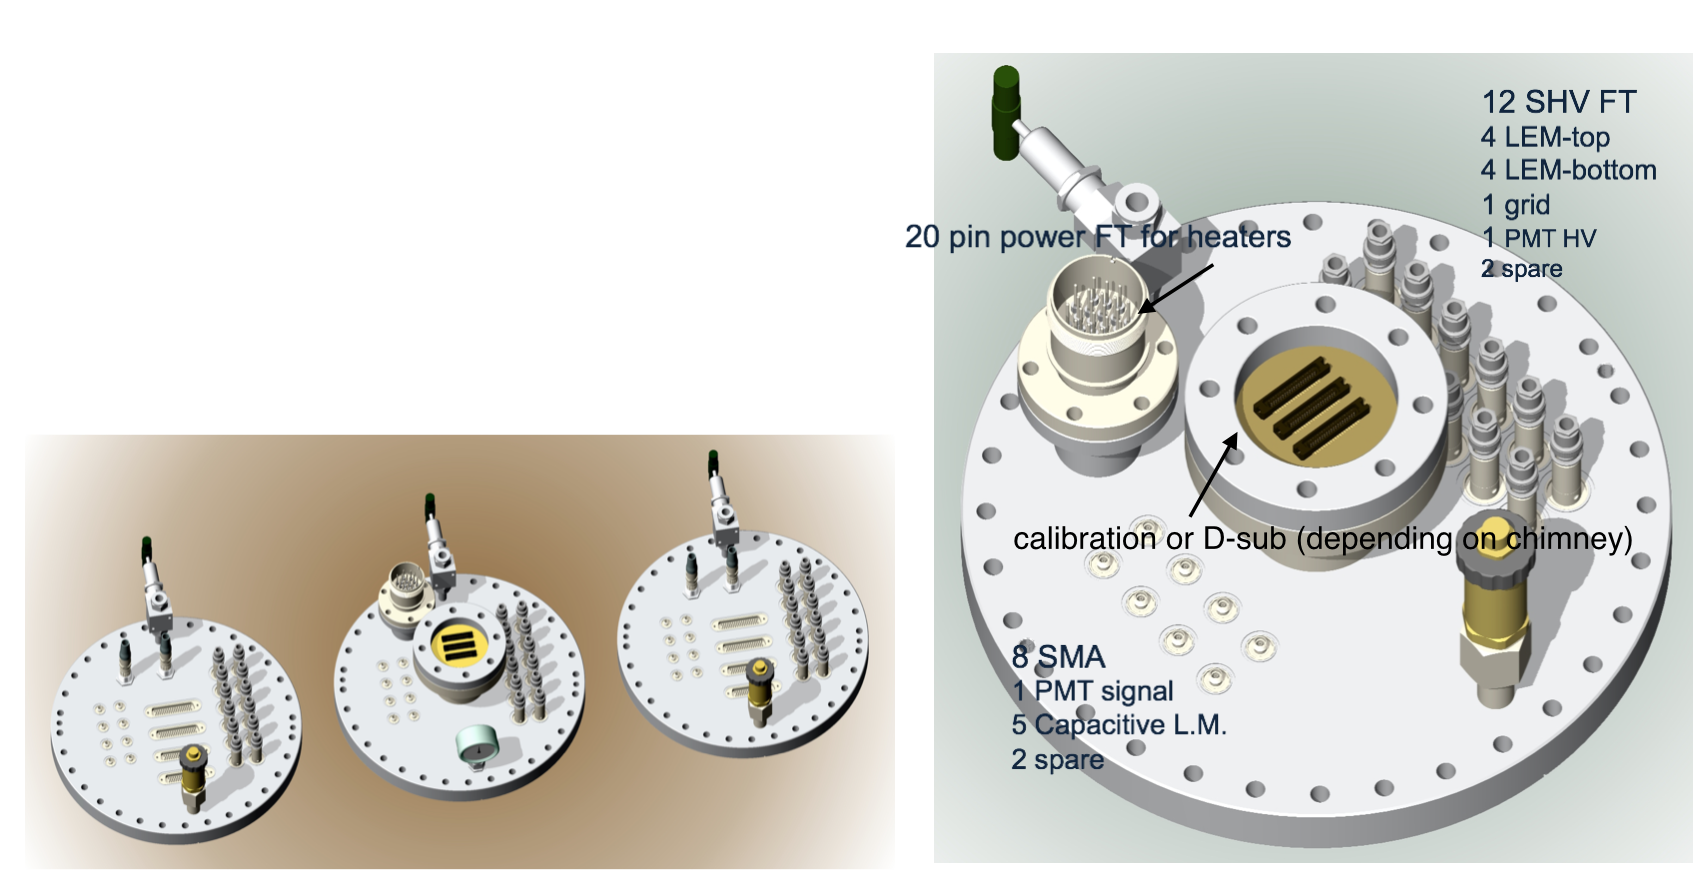
\includegraphics[scale=0.52, angle=0]{SC_flange.png}
 \end{cdrfigure}

\begin{cdrfigure}[List of the slow control sensors for  the $3 \times 1 \times 1$ $m^2$ prototype and far detector detectors.]{sc_sensors}{List of the slow control sensors for the $3 \times 1 \times 1$ $m^2$ prototype and far detector detectors.}
 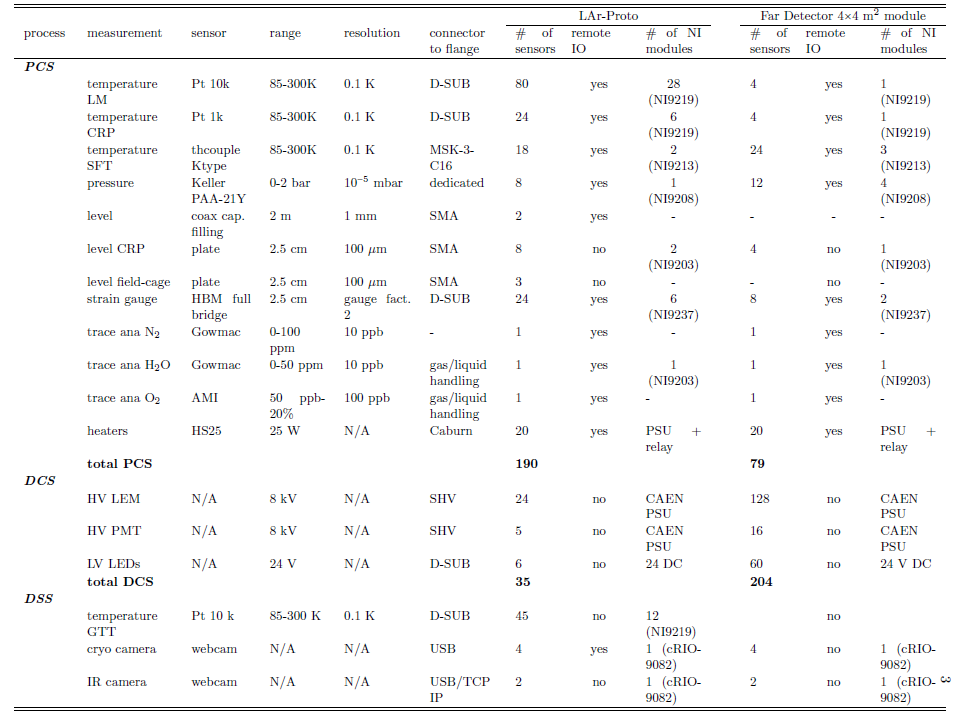
\includegraphics[scale=0.6, angle=0]{sc_table.png} %[scale=0.52, angle=0]{sc_table.png}
 \end{cdrfigure}
   